% Тип документа
\documentclass[a4paper,12pt]{extarticle}

% Шрифты, кодировки, символьные таблицы, переносы
\usepackage{cmap}
\usepackage[T2A]{fontenc}
\usepackage[utf8x]{inputenc}
\usepackage[russian]{babel}

% Это пакет -- хитрый пакет, он нужен но не нужен
\usepackage[mode=buildnew]{standalone}

\usepackage
	{
		% Дополнения Американского математического общества (AMS)
		amssymb,
		amsfonts,
		amsmath,
		amsthm,
		physics,
		% misccorr,
		% 
		% Графики и рисунки
		wrapfig,
		graphicx,
		subcaption,
		float,
		tikz,
		tikz-3dplot,
		caption,
		csvsimple,
		color,
		booktabs,
		pgfplots,
		pgfplotstable,
		geometry,
		% 
		% Таблицы, списки
		array,
		makecell,
		multirow,
		indentfirst,
		%
		% Интегралы и прочие обозначения
		ulem,
		esint,
		esdiff,
		% 
		% Колонтитулы
		fancyhdr,
	}  

\usepackage{xcolor}
\usepackage{hyperref}

 % Цвета для гиперссылок
\definecolor{linkcolor}{HTML}{000000} % цвет ссылок
\definecolor{urlcolor}{HTML}{799B03} % цвет гиперссылок
 
\hypersetup{pdfstartview=FitH,  linkcolor=linkcolor,urlcolor=urlcolor, colorlinks=true}
% Обводка текста в TikZ
\usepackage[outline]{contour}

% Увеличенный межстрочный интервал, французские пробелы
\linespread{1.3} 
\frenchspacing 

 
\usetikzlibrary
	{
		decorations.pathreplacing,
		decorations.pathmorphing,
		patterns,
		calc,
		scopes,
		arrows,
		fadings,
		through,
		shapes.misc,
		arrows.meta,
		3d,
		quotes,
		angles,
		babel
	}


\tikzset{
	force/.style=	{
		>=latex,
		draw=blue,
		fill=blue,
				 	}, 
	%				 	
	axis/.style=	{
		densely dashed,
		blue,
		line width=1pt,
		font=\small,
					},
	%
	th/.style=	{
		line width=1pt},
	%
	acceleration/.style={
		>=open triangle 60,
		draw=magenta,
		fill=magenta,
					},
	%
	inforce/.style=	{
		force,
		double equal sign distance=2pt,
					},
	%
	interface/.style={
		pattern = north east lines, 
		draw    = none, 
		pattern color=gray!60,
					},
	cross/.style=	{
		cross out, 
		draw=black, 
		minimum size=2*(#1-\pgflinewidth), 
		inner sep=0pt, outer sep=0pt,
					},
	%
	cargo/.style=	{
		rectangle, 
		fill=black!70, 
		inner sep=2.5mm,
					},
	%
	caption/.style= {
		midway,
		fill=white!20, 
		opacity=0.9
					},
	%
	}

\newenvironment{tikzpict}
    {
	    \begin{figure}[htbp]
		\centering
		\begin{tikzpicture}
    }
    { 
		\end{tikzpicture}
		% \caption{caption}
		% \label{fig:label}
		\end{figure}
    }


\newcommand{\vbLabel}[3]{\draw ($(#1,#2)+(0,5pt)$) -- ($(#1,#2)-(0,5pt)$) node[below]{#3}}
\newcommand{\vaLabel}[3]{\draw ($(#1,#2)+(0,5pt)$) node[above]{#3} -- ($(#1,#2)-(0,5pt)$) }

\newcommand{\hrLabel}[3]{\draw ($(#1,#2)+(5pt,0)$) -- ($(#1,#2)-(5pt,0)$) node[right, xshift=1em]{#3}}
\newcommand{\hlLabel}[3]{\draw ($(#1,#2)+(5pt,0)$) node[left, xshift=-1em]{#3} -- ($(#1,#2)-(5pt,0)$) }



\newcommand\zi{^{\,*}_i}
\newcommand\sumn{\sum_{i=1}^{N}}

\tikzset{
	coordsys/.style={scale=1.8,x={(1.1cm,-0cm)},y={(0.5cm,1cm)}, z={(0cm,0.8cm)}},
	coordsys/.style={scale=1.5,x={(0cm,0cm)},y={(1cm,0cm)}, z={(0cm,1cm)}}, 
	coordsys/.style={scale=1.5,x={(1cm,0cm)},y={(0cm,1cm)}, z={(0cm,0cm)}}, 
}

\usepgfplotslibrary{units}


% Draw line annotation
% Input:
%   #1 Line offset (optional)
%   #2 Line angle
%   #3 Line length
%   #5 Line label
% Example:
%   \lineann[1]{30}{2}{$L_1$}

\newcommand{\lineann}[4][0.5]{%
    \begin{scope}[rotate=#2, blue,inner sep=2pt, ]
        \draw[dashed, blue!40] (0,0) -- +(0,#1)
            node [coordinate, near end] (a) {};
        \draw[dashed, blue!40] (#3,0) -- +(0,#1)
            node [coordinate, near end] (b) {};
        \draw[|<->|] (a) -- node[fill=white, scale=0.8] {#4} (b);
    \end{scope}
}

\newcommand{\lineannn}[4][0.5]{%
    \begin{scope}[rotate=#2, blue,inner sep=2pt, ]
        \draw[dashed, blue!40] (0,0) -- +(0,#1)
            node [coordinate, near end] (a) {};
        \draw[dashed, blue!40] (#3,0) -- +(0,#1)
            node [coordinate, near end] (b) {};
        % \draw[color=white, color=blue] (a) -- node[fill=white, scale=0.8] {#4} (b);
        \draw[->|] (a)++(-0.3,0) -- (a);
        \draw[->|] (b)++(0.3,0) coordinate (xx) -- (b);
        \draw (xx) node[fill=white, scale=0.8, right] {#4};
    \end{scope}
}

% Круговая стрелка относительно центра (дуга из центра)
\tikzset{
  pics/carc/.style args={#1:#2:#3}{
    code={
      \draw[pic actions] (#1:#3) arc(#1:#2:#3);
    }
  },
  dash/.style={
  	dash pattern=on 5mm off 5mm
  }
}

% Среднее <#1>
\newcommand{\mean}[1]{\langle#1\rangle}

\pgfplotsset{
    % most recent feature set of pgfplots
    compat=newest,
}

% const прямым шрифтом
\newcommand\ct[1]{\text{\rmfamily\upshape #1}}
\newcommand*{\const}{\ct{const}}


\usepackage[europeanresistors,americaninductors]{circuitikz}

% Style to select only points from #1 to #2 (inclusive)
\pgfplotsset{select/.style 2 args={
    x filter/.code={
        \ifnum\coordindex<#1\def\pgfmathresult{}\fi
        \ifnum\coordindex>#2\def\pgfmathresult{}\fi
    }
}}


\usepackage{array}
\usepackage{pstool}


%%%%%%%%%%%%%%%%%%%%%%%%%%%%%%%%%%%%%%%%%%%%%%%%%
\makeatletter
\newif\if@gather@prefix 
\preto\place@tag@gather{% 
  \if@gather@prefix\iftagsleft@ 
    \kern-\gdisplaywidth@ 
    \rlap{\gather@prefix}% 
    \kern\gdisplaywidth@ 
  \fi\fi 
} 
\appto\place@tag@gather{% 
  \if@gather@prefix\iftagsleft@\else 
    \kern-\displaywidth 
    \rlap{\gather@prefix}% 
    \kern\displaywidth 
  \fi\fi 
  \global\@gather@prefixfalse 
} 
\preto\place@tag{% 
  \if@gather@prefix\iftagsleft@ 
    \kern-\gdisplaywidth@ 
    \rlap{\gather@prefix}% 
    \kern\displaywidth@ 
  \fi\fi 
} 
\appto\place@tag{% 
  \if@gather@prefix\iftagsleft@\else 
    \kern-\displaywidth 
    \rlap{\gather@prefix}% 
    \kern\displaywidth 
  \fi\fi 
  \global\@gather@prefixfalse 
} 
\newcommand*{\beforetext}[1]{% 
  \ifmeasuring@\else
  \gdef\gather@prefix{#1}% 
  \global\@gather@prefixtrue 
  \fi
} 
\makeatother
%%%%%%%%%%%%%%%%%%%%%%%%%%%%%%%%%%%%%%%%%%%%%%%%%

\geometry		
	{
		left			=	2cm,
		right 			=	2cm,
		top 			=	3cm,
		bottom 			=	3cm,
		bindingoffset	=	0cm
	}

%%%%%%%%%%%%%%%%%%%%%%%%%%%%%%%%%%%%%%%%%%%%%%%%%%%%%%%%%%%%%%%%%%%%%%%%%%%%%%%



	%применим колонтитул к стилю страницы
\pagestyle{fancy} 
	%очистим "шапку" страницы
\fancyhead{} 
	%слева сверху на четных и справа на нечетных
\fancyhead[R]{\labauthors} 
	%справа сверху на четных и слева на нечетных
\fancyhead[L]{Отчёт по лабораторной работе №\labnumber} 
	%очистим "подвал" страницы
\fancyfoot{} 
	% номер страницы в нижнем колинтуле в центре
\fancyfoot[C]{\thepage} 

%%%%%%%%%%%%%%%%%%%%%%%%%%%%%%%%%%%%%%%%%%%%%%%%%%%%%%%%%%%%%%%%%%%%%%%%%%%%%%%

\renewcommand{\contentsname}{Оглавление}

\usepackage{tocloft}
% \renewcommand{\cftpartleader}{\cftdotfill{\cftdotsep}} % for parts
% \renewcommand{\cftsectiondotsep}{\cftdotsep}% Chapters should use dots in ToC
\renewcommand{\cftsecleader}{\cftdotfill{\cftdotsep}}
%\renewcommand{\cftsecleader}{\cftdotfill{\cftdotsep}} % for sections, if you really want! (It is default in report and book class (So you may not need it).
% ---------
% \newcommand{\cftchapaftersnum}{.}%
% \usepackage{titlesec}
% \titlelabel{\thetitle.\quad}
\usepackage{secdot}
\sectiondot{subsection}

\renewcommand{\phi}{\varphi}

\begin{document}

\def\labauthors{Виноградов И.Д., Шиков А.П.}
\def\labgroup{430}
\def\labnumber{1}
\def\labtheme{Измерение ширины запрещенной зоны}
\begin{titlepage}

\begin{center}

{\small\textsc{Нижегородский государственный университет имени Н.\,И. Лобачевского}}
\vskip 1pt \hrule \vskip 3pt
{\small\textsc{Радиофизический факультет. Кафедра Радиотехники.}}

\vfill

{\Large Отчет по лабораторной работе №\labnumber\vskip 12pt\bfseries \labtheme}
	
\end{center}

\vfill
	
\begin{flushright}
	{Выполнили студенты \labgroup\ группы\\ \labauthors}%\vskip 12pt Принял:\\ Менсов С.\,Н.}
\end{flushright}
	
\vfill
	
\begin{center}
	Нижний Новгород, \the\year
\end{center}

\end{titlepage}



% \tableofcontents

\newpage
\section*{Введение}
Ширина запрещенной зоны является одной из важнейших характеристик полупроводниковых материалов. Она может быть найдена
по результатам измерений электропроводности или постоянной Холла в зависимости от температуры, а также из спектрального 
распределения коэффициента оптического поглощения или фототока полупроводника. В настоящей работе студентам предлагается
определить величину ширины запрещенной зоны полупроводникового материала по результатам измерения температурной зависимости 
электропроводности. 

\section{Элементы зонной теории полупроводников}
В изолированном атоме электроны находятся в стационарных состояниях, каждому из которых соответствует строго
определенное значение энергии. Таким образом, энергетический спектр электронных состояний в атоме является дискретным. В
кристаллическом твердом теле из-за возмущений, вносимых другими атомами, уровни энергии расщепляются – образуются
области или зоны разрешенных значений энергии, между которыми находятся запрещенные зоны. Для глубоких уровней
расщепление невелико, т.к. находящиеся на них электроны экранируются верхними оболочками и практически не
взаимодействуют с соседними атомами. Для внешних оболочек расщепление может составлять несколько электрон-вольт. 

Поскольку энергетические зоны образованы из соответствующих уровней изолированных атомов, то общее число электронов,
которые могут разместиться в данной зоне, равно общему числу мест на уровнях изолированных атомов, из которых образован
кристалл. Если при абсолютном нуле температур осуществлять заполнение зон электронами, то заселение энергетических
уровней будет осуществляться снизу вверх и на каждом уровне, согласно принципу Паули, будут располагаться два электрона,
что соответствует двум различным ориентация спина. Самая верхняя полностью заполненная при абсолютном нуле температуры
электронами зона называется валентной. Ближайшая к ней незаполненная или частично заполненная зона называется зоной
проводимости. Как правило, в рассмотрении участвуют именно эти две зоны, поскольку все более глубоко лежащие полностью
заполнены электронами и, следовательно, вклад в проводимость не дают (все уровни заняты, т.е. изменение энергии заряда,
обусловленное приложением электрического поля, невозможно). Таким образом, упрощенная структура энергетического спектра
электронов в твердом теле будет иметь вид, представленный на рис. \ref{fig:cond}. Расстояние между дном зоны проводимости и
потолком валентной зоны называют шириной запрещенной зоны. 

\begin{wrapfigure}{l}{0.5\linewidth}
	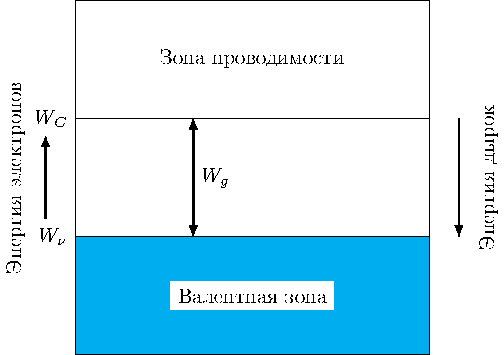
\includegraphics[width = \linewidth]{img/cond.pdf}
	\caption{Энергитический спектр электрона в кристалле. $W_c,W_{\nu}$ - соответственно, энергии дна зоны проводимости и потолка валентной зоны, $W_g$ - ширина запрещенной зоны.}
	\label{fig:cond}
\end{wrapfigure}

Представление о разрешенных и запрещенных зонах в сочетании с принципом Паули позволяет понять причину глубокого
различия физических свойств металлов, диэлектриков и полупроводников. Действительно, если при абсолютном нуле зона
проводимости полупроводника частично заполнена электронами или имеется перекрытие заполненной валентной зоны и пустой
зоны проводимости, то в случае приложения электрического поля будут осуществляться энергетические переходы,
обусловленные ускорением электронов во внешнем поле. Такие материалы проводят электрический ток даже при абсолютном нуле
температуры и являются металлами.  
 
Теперь рассмотрим ситуацию, когда между валентной зоной и зоной проводимости имеется запрещенная зона конечной ширины
(рис. \ref{fig:cond}). В этом случае при абсолютном нуле, а также полном затемнении и не слишком сильном электрическом поле твердое
тело не будет проводить электрический ток: в зоне проводимости электронов нет, а электроны заполненной валентной зоны не
могут изменить своего состояния, поскольку все соседние уровни заняты. При повышении температуры и/или освещении такого
тела электроны валентной зоны будут получать дополнительную энергию и переходить в зону проводимости. Вследствие таких
переходов, во-первых, появятся электроны в зоне проводимости (они будут участвовать в переносе тока и обеспечивать
электронную проводимость), а во-вторых, освободятся верхние уровни валентной зоны, что позволит и ее электронам
участвовать в переносе тока, обеспечивая дырочную проводимость. Материал, имеющий запрещенную зону небольшой ширины,
является полупроводником. Разница между полупроводниками и диэлектриками с точки зрения зонной теории заключается лишь в
величине ширины запрещенной зоны.

Ширина запрещенной зоны $W_g$  – один из важнейших параметров твердотельных материалов.
При температуре 300 К она составляет в германии (Ge) 0.803 эВ, в кремнии (Si) – 1.12 эВ, в арсениде галлия (GaAs) – 1.43
эВ, в фосфиде индия (InP) – 1.29 эВ.

\subsection{Краткое описание кристаллической структуры полупроводников}
Надо? да, но в конце.

\section{Концентрация носителей заряда в полупроводнике}
Вычисление концентрации подвижных и связанных носителей заряда в полупроводнике составляет задачу статистики электронов.
Решение этой задачи, с одной стороны, позволяет объяснить экспериментальные результаты, по которым, в свою очередь,
становится возможным определение ряда важных характеристик полупроводника (ширины запрещенной зоны, энергия ионизации примеси).
Задача вычисления концентрации носителей заряда распадается на две:  1) определение числа возможных квантовых состояний
электронов в разрешенных зонах в твердом теле и 2) выяснение фактического распределения электронов по этим квантовым
состояниям. Рассмотрим последовательно решение каждой из подзадач.

Число состояний в любой зоне кристалла равно общему числу мест на уровнях изолированных атомов, образовавших кристалл,
т.е. числу атомов $N_0$, умноженному на кратность вырождения $\nu$ атомного уровня, образовавшего данную зону:

\begin{equation}
	\int \limits_{W_1}^{W_2} N(W) dW  =\nu N_0 
	\label{eq:1}
\end{equation} 

где $N(W)dW$ - число  квантовых состояний в интервале энергий от $W$ до $W+dW$ в единице объёма полупроводника, а $N(W)$
-  плотность квантовых состояний. $W_1,W_2$ - энергии нижнего и верхнего края зоны, соответственно. 

Нахождение точного вида функции $N(W)$ – очень сложная задача. Приведем ее решение для простейшего случая, когда электроны
заполняют только уровни вблизи дна зоны проводимости, т.е. для описания зависимости энергии носителей от квазиимпульса
$W(~\vec{p}~)$ справедливо приближение эффективной массы:   
\begin{equation}
	W = W_C + \frac{p^2}{2m_n^*}
	\label{eq:2}
\end{equation}

где $W_C$ – энергия дна зоны проводимости, $m_n^*$ –  эффективная масса электрона на дне зоны проводимости, $\vec{p} =
\hbar \vec{k}$ – квазиимпульс электрона, $\vec{k}$ – квазиволновой вектор. Число состояний в интервале энергий $(W, W+dW)$ может быть найдено
путем определения отношения объема в пространстве квазиволновых векторов (kпространстве), заключенного между двумя
указанными изоэнергетическими поверхностями, к объему одного квантового состояния. 

В случае закона дисперсии, представленного в виде \eqref{eq:2} поверхности равной энергии в k-пространстве являются
сферами с радиусом k. Выделим шаровой слой, заключенный между двумя изоэнергетическими поверхностями, соответствующими
энергиям $W$ и $W+dW$. Объем этого слоя имеет величину: 
\begin{equation}
	dV_p = 4 \pi k^2 d k
	\label{eq:3}
\end{equation}
Объём, приходящийся на одно электронное состояние равен $dk_x dk_y dk_z = \frac{(2 \pi)^3}{V}$ , где $V$ – объём
кристалла. В каждой ячейке могут находиться два электрона с противоположными спинами. С учетом этого, число состояний в
объеме $dV_p$ равно: 
\begin{equation}
	d Z=2 \frac{d V_{p}}{(2 \pi \hbar)^{3}}=\frac{k^{2} d k}{\pi^{2}}
	\label{eq:4}
\end{equation}
Из равенства \eqref{eq:2} получаем: 
\begin{equation}
	\hbar k=\sqrt{2 m_{n}^{*}\left(W-W_{C}\right)}
	\label{eq:5}
\end{equation}
откуда:
\begin{equation}
	d k=\frac{1}{2 \hbar}\left(2 m_{n}^{*}\left(W-W_{C}\right)\right)^{-1 / 2} d W
	\label{eq:6}
\end{equation}
Подставляя \eqref{eq:5} и \eqref{eq:6} в \eqref{eq:4}, получим выражение для плотности квантовых состояний у дна зоны
проводимости:
\begin{equation}
	N_{c}(W)=\frac{d Z}{d W}=4 \pi\left[\frac{2 m_{n}^{*}}{(2 \pi \hbar)^{2}}\right]^{3 / 2} \sqrt{W-W_{C}}
	\label{eq:7}
\end{equation} 
Аналогично определяется плотность состояний вблизи потолка валентной зоны.

Для определения числа электронов в зоне проводимости или дырок в валентной зоне кроме плотности состояний необходимо
знать также вероятность заполнения каждого состояния (уровня энергии) электронами. Если считать электроны
невзаимодействующими, как это обычно делается, то газ электронов подчиняется законам идеального газа. 

Статистика электронов подчиняется распределению Ферми-Дирака:   
\begin{equation}
	f(W) = \frac{1}{exp (\frac{W-W_F}{k_B T})+1}
	\label{eq:8}
\end{equation}
которое даёт вероятность того, что в тепловом равновесии состояние с энергией $W$ занято электроном. Здесь $k_B$ –
постоянная Больцмана, $Т$ – абсолютная температура, $W_F$ – энергия (уровень) Ферми – максимальная энергия электронов при
абсолютном нуле. Для температуры, отличной от нуля, функция $f(W)$ в точке $W = W_F$ имеет перегиб. Рассмотрим случай,
когда $Т > 0$. Из выражения \eqref{eq:8} следует, что для $W=W_F: f(W) =1/2$. При очень больших энергиях, когда $ W-W_F
>> k_B T $, можно пренебречь 1 в знаменателе, и выражение $f(W)$ принимает вид:
\begin{equation}
	f(W) = exp (\frac{W_F-W}{k_B T})
	\label{eq:9}
\end{equation} 
т.е. совпадает с функцией Максвелла-Больцмана для частиц, подчиняющихся классическим законам. Аналогично, при очень
малых энергиях, когда $W<<W_F$ (но $W-W_F>>k_B T$), экспонента в знаменателе \eqref{eq:8} очень мала и, разлагая функцию $f(W)$ в ряд по
малому параметру и ограничиваясь нулевым и первым слагаемыми, получим: 
\begin{equation}
	f(W) = 1 - exp( \frac{W-W_F}{k_BT})
	\label{eq:10}
\end{equation}
Зависимость плотности состояний в зоне проводимости от энергии и вероятности заполнения этих состояний позволяет
определить концентрацию свободных электронов $dn$, энергия которых заключена в интервале от $W$ до $W+dW$:
\begin{equation}
	dn = f(W) N(W)dW
	\label{eq:11}
\end{equation}
Интегрирование выражения \eqref{eq:11} по всей зоне проводимости позволяет найти полное число электронов в ней. Так как функция
Ферми быстро спадает с ростом энергии, верхний предел можно заменить бесконечностью. 

В элементарных функциях такой интеграл не вычисляется, и для его нахождения используют специальные таблицы. Однако, если
уровень Ферми лежит в запрещенной зоне достаточно далеко от ее краев, т.е. $W_c - W_F>>k_B T$ , то для функции Ферми
справедливо приближение Больцмана и интеграл можно вычислить. Такой полупроводник называется невырожденным. Интегрируя
\eqref{eq:11} в данном приближении, получим: 
\begin{equation}
	n=\int_{W_{C}}^{\infty} f(W) N(W) d W=N_{c} exp(-\frac{W_C-W_F}{k_B T})
	\label{eq:12}
\end{equation}
где $N_{c}=2\left[\frac{2 \pi m_{n}^{*} k_{B} T}{h^{2}}\right]^{3 / 2}$ - эффективная плотность состояний в зоне проводи
мости.

Аналогично концентрация дырок: 
\begin{equation}
	p=N_{\nu} e^{-\frac{W_{F}-W_{\nu}}{k_{B} T}}
	\label{eq:13}
\end{equation}
где $N_{\nu}=2\left[\frac{2 \pi m_{p}^{*} k_{B} T}{h^{2}}\right]^{3 / 2}$ - эффективная плотность состояний валентной зоне.

Полученные выше выражения для концентрации электронов и дырок в совокупности с принципом электронейтральности
полупроводника ( в однородном полупроводнике не может быть существенных нескомпенсированных объемных зарядов ни в
равновесном состоянии, ни при наличии тока ) позволяют сделать выводы о положении уровня Ферми в полупроводнике.
Рассмотрим собственный полупроводник, для которого влияние примесных атомов не существенно. Свободные носители заряда в
этом случае возникают только за счет разрыва валентных связей. Поэтому в собственном полупроводнике концентрация дырок p
равна концентрации электронов $ n: n = p \equiv n_i$. Это условие электронейтральности собственного полупроводника. Из этого
условия, приравняв \eqref{eq:12} и \eqref{eq:12}, получим:
\begin{equation}
	W_{F}=\frac{W_{c}+W_{v}}{2}+\frac{k_{B} T}{2} \ln \frac{N_{V}}{N_{c}}=\frac{W_{c}+W_{v}}{2}-\frac{3 k_{B} T}{4} \ln \frac{m_{n}^{*}}{m_{p}^{*}}
	\label{eq:14}
\end{equation}
т.е. уровень Ферми $W_F$ собственного полупроводника при абсолютном нуле температуры лежит в центре запрещенной зоны и,
вообще говоря, смещается при возрастании температуры. Этот случай показан на рис.(??), где слева направо схематически
приведены простейшая зонная диаграмма, плотность состояний $N(W)$, распределение Ферми $f (W)$ и концентрация носителей
заряда.

Если в полупроводник введены примесные атомы, то, как показано на рис. 2.1.б и 2.1.в (??), уровень Ферми должен смещаться для
сохранения электронейтральности. В случае 2.1.б(??), например, в кристалл добавляется донорная примесь, приводящая к
образованию локальных энергетических уровней Wd. Пусть концентрация доноров составляет $N_d$ (см$^{-3}$). Для сохранения
элентронейтральности отрицательный заряд электронов должен быть равен полному заряду дырок и ионизованных доноров:
\begin{equation}
	n = N_d+p
	\label{eq:15}
\end{equation}
Следовательно, $n>р$ и уровень Ферми обязан сместиться к дну зоны проводимости, как показано на рис. 2.1.б.

Температурная зависимость концентраций электронов и дырок в собственном полупроводнике определяется формулами \eqref{eq:12} и \eqref{eq:13} с учетом
\eqref{eq:14}. Этими же формулами определяются и концентрации носителей в примесном полупроводнике при достаточно высоких
температурах, когда количество электронов в зоне проводимости и дырок в валентной зоне определяется переходами
электронов через запрещенную зону. При этом уровень Ферми лежит вблизи середины запрещенной зоны, т.е. $W_F =
\frac{W_c+W_{\nu}}{2}$. Подставляя последнее соотношение в \eqref{eq:12}, получим концентрацию электронов:
\begin{equation}
	n=N_{c} e^{-\frac{W_{c}-W_{v}}{2 k_{B} T}}=N_{c} e^{-\frac{W_{g}}{2 k_{B} T}}
	\label{eq:16}
\end{equation}
где $W_g$  – ширина запрещенной зоны. Величина $N_c$ зависит от температуры по закону $Т^{3/2}$. Эта зависимость слабая по
сравнению с экспонентой, поэтому температурная зависимость концентрации определяется, в основном, экспоненциальным
множителем. 

При низких температурах концентрация носителей в примесном полупроводнике определяется примесями. При очень низких
температурах, когда еще не вся примесь ионизована, уровень Ферми, например, для электронного полупроводника, лежит
примерно посередине между уровнем донорной примеси и дном зоны проводимости, т.е. $W_F = \frac{W_c+W_{d}}{2}$. Тогда \eqref{eq:12}
принимает вид: 
\begin{equation}
	n=N_{c} e^{-\frac{W_{c}-W_{d}}{2 k_{B} T}}=N_{c} e^{-\frac{\Delta W_{d}}{2 k_{B} T}}
	\label{eq:17}
\end{equation}
где $\Delta W_d$ – энергия ионизации донорной примеси. 


Для более высоких температур, когда вся примесь ионизована, но вероятность перехода электронов из валентной зоны мала,
концентрация носителей заряда просто равна концентрации примеси $n=N_d$. 
%%%%%%%%%%%%%%%%%%%%%%%%%%%%%%%%%%%%%%%%%%%%%%%%%%%%%%%%%%%%%%%%%%%%%%%%%%%%%%%%%%%%%%%%%%%%%%%%%%%%%%%%%%%
%%%%%%%%%%%%%%%%%%%%%%%%%%%%%%%%%%%%%%%%%%%%%%%%%%%%%%%%%%%%%%%%%%%%%%%%%%%%%%%%%%%%%%%%%%%%%%%%%%%%%%%%%%%
%%%%%%%%%%%%%%%%%%%%%%%%%%%%%%%%%        КАРТИНКУ        %%%%%%%%%%%%%%%%%%%%%%%%%%%%%%%%%%%%%%%%%%%%%%%%%%
%%%%%%%%%%%%%%%%%%%%%%%%%%%%%%%%%%%%%%%%%%%%%%%%%%%%%%%%%%%%%%%%%%%%%%%%%%%%%%%%%%%%%%%%%%%%%%%%%%%%%%%%%%%
%%%%%%%%%%%%%%%%%%%%%%%%%%%%%%%%%%%%%%%%%%%%%%%%%%%%%%%%%%%%%%%%%%%%%%%%%%%%%%%%%%%%%%%%%%%%%%%%%%%%%%%%%%%

Таким образом, зависимость концентрации от температуры имеет три участка (см. рис. 2.2.). Область примесной проводимости
при низких температурах – 1-2; область истощения примесей – участок 2-3 и область собственной проводимости – участок
3-4. В координатах $ln(n)$, $1/T$ экспоненты (2.16), (2.17.) выглядят как прямые, наклон которых характеризуется величинами
$W_g$ и $\Delta W_d$. Результаты измерения температурной зависимости концентрации электронов позволяют определить ширину
запрещенной зоны полупроводника и энергию ионизации примеси.

%%%%%%%%%%%%%%%%%%%%%%%%%%%%%%%%%%%%%%%%%%%%%%%%%%%%%%%%%%%%%%%%%%%%%%%%%%%%%%%%%%%%%%%%%%%%%%%%%%%%%%%%%%%
%%%%%%%%%%%%%%%%%%%%%%%%%%%%%%%%%%%%%%%%%%%%%%%%%%%%%%%%%%%%%%%%%%%%%%%%%%%%%%%%%%%%%%%%%%%%%%%%%%%%%%%%%%%
%%%%%%%%%%%%%%%%%%%%%%%%%%%%%%%%%        КАРТИНКУ        %%%%%%%%%%%%%%%%%%%%%%%%%%%%%%%%%%%%%%%%%%%%%%%%%%
%%%%%%%%%%%%%%%%%%%%%%%%%%%%%%%%%%%%%%%%%%%%%%%%%%%%%%%%%%%%%%%%%%%%%%%%%%%%%%%%%%%%%%%%%%%%%%%%%%%%%%%%%%%
%%%%%%%%%%%%%%%%%%%%%%%%%%%%%%%%%%%%%%%%%%%%%%%%%%%%%%%%%%%%%%%%%%%%%%%%%%%%%%%%%%%%%%%%%%%%%%%%%%%%%%%%%%%
Измерение концентрации носителей заряда требует разработки специальной методики. Гораздо проще проводить измерения
проводимости образца, но на нее, помимо концентрации носителей, оказывает влияние подвижность частиц. Поэтому далее мы
разберем особенности движения носителей заряда в полупроводнике под действием электрического поля. 


\section{Подвижность носителей заряда в полупроводнике}


\section{Температурная зависимость проводимости}
В реальной кристаллической структуре всегда присутствуют дефекты: тепловые колебания атомов решётки, примеси и т.д.
Поэтому при воздействии внешнего электрического поля частица движется ускоренно лишь на небольшом участке пути, а затем
испытывает рассеяние (взаимодействие с дефектами кристалла), изменяя свой импульс и ( в случае неупругого
взаимодействия) энергию, теряет направленную скорость, после чего процесс разгона начинается заново (рис. 3.1). В слабых
электрических полях ($\leq 10^3$ В/см) средняя скорость направленного движения носителей заряда (дрейфовая скорость)
пропорциональна напряжённости электрического поля:$\nu = \mu E$. Коэффициент пропорциональности между скоростью и полем $\mu$
называется подвижностью носителей заряда. Эта величина численно равна средней скорости направленного движения частиц в
электрическом поле с напряженностью 1 В/м. 
%%%%%%%%%%%%%%%%%%%%%%%%%%%%%%%%%%%%%%%%%%%%%%%%%%%%%%%%%%%%%%%%%%%%%%%%%%%%%%%%%%%%%%%%%%%%%%%%%%%%%%%%%%%
%%%%%%%%%%%%%%%%%%%%%%%%%%%%%%%%%%%%%%%%%%%%%%%%%%%%%%%%%%%%%%%%%%%%%%%%%%%%%%%%%%%%%%%%%%%%%%%%%%%%%%%%%%%
%%%%%%%%%%%%%%%%%%%%%%%%%%%%%%%%%        КАРТИНКУ        %%%%%%%%%%%%%%%%%%%%%%%%%%%%%%%%%%%%%%%%%%%%%%%%%%
%%%%%%%%%%%%%%%%%%%%%%%%%%%%%%%%%%%%%%%%%%%%%%%%%%%%%%%%%%%%%%%%%%%%%%%%%%%%%%%%%%%%%%%%%%%%%%%%%%%%%%%%%%%
%%%%%%%%%%%%%%%%%%%%%%%%%%%%%%%%%%%%%%%%%%%%%%%%%%%%%%%%%%%%%%%%%%%%%%%%%%%%%%%%%%%%%%%%%%%%%%%%%%%%%%%%%%%

Подвижность носителей заряда сильно меняется с изменением температуры. Для получения этой зависимости необходимо кратко
остановится на основных механизмах рассеяния носителей заряда в полупроводниках. 

Рассеяние носителей заряда на нейтральных атомах примеси и нейтральных дефектах является слабым. Однако, при низких
температурах, когда примеси еще практически не ионизованы, а тепловые колебания отсутствуют, этот механизм играет
существенную роль. Для того, чтобы электрон изменил направление своего движения в результате взаимодействия с
нейтральной примесью или дефектом, необходимо, чтобы траектория электрона проходила через место расположения дефекта
либо через примыкающую к нему область решетки, в которой им вызваны искажения. Рассеяние на нейтральных примесях не
зависит от температуры, а подвижность, обусловленная этим рассеянием, постоянна и зависит только от концентрации
рассеивающих центров.

Электрическое поле ионизованного примесного атома распространяется на много периодов кристаллической решетки, и
электрон, проходя на значительном расстоянии от иона, изменит под действием его поля направление своего движения. Пусть
рассеяние в полупроводнике происходит только на ионах примеси, а тепловые колебания и нейтральные центры рассеяния
отсутствуют. Тогда, как показывают расчеты, подвижность зависит от температуры как $Т^{3/2}$, т.е. увеличивается. Этот
результат легко понять, если учесть, что с ростом температуры увеличивается средняя скорость хаотического движения
электронов, а быстрые электроны слабее отклоняются статическим полем ионов. Этот механизм рассеяния играет основную роль
при температурах, когда уже имеется большая концентрация ионизированных примесей, но тепловые колебания еще мало влияют
на рассеяние. 

Рассмотрим теперь полупроводник, в котором отсутствуют примеси и дефекты, а рассеяние происходит только на тепловых
колебаниях решетки. С ростом температуры амплитуда колебаний возрастает или, говоря языком квантовой статистики,
возрастает концентрация фононов в кристалле. Очевидно, что рассеяние с ростом температуры должно усиливаться, а
подвижность падать. Для неполярных полупроводников, таких как германий и кремний, уменьшение подвижности происходит по
закону $Т^{3/2}$. 

Если же действует одновременно все три механизма рассеяния, то результирующая подвижность будет определяться так: 
\begin{equation}
	\frac{1}{\mu_{\Sigma}} = \frac{1}{\mu_{1}}+\frac{1}{\mu_{2}}+\frac{1}{\mu_{3}}
	\label{eq:3.1}
\end{equation}

Поскольку подвижность – это средняя скорость в единичном электрическом поле, то она пропорциональна среднему времени
свободного пробега $\tau$, за которое электрон набирает направленную скорость. Если $\tau_1, \tau_2,\tau_3$ – времена свободного
пробега для каждого из трех механизмов рассеяния, то $1/\tau_1,1/\tau_2,1/\tau_3$ – соответствующие частоты столкновений. Когда
действует несколько механизмов рассеяния, то эти частоты складываются арифметически, откуда и следует формула (3.1). Для
выполнения данной работы важно, что итоговая зависимость подвижности от температуры является степенной функцией.


\section{Схема установки и методика измерений}

\section*{Эксперимент}
 

\end{document}
